\chapter{Methodology Part 2: Advancing Several Layers}

In the previous chapter, we talked about how the very first layer of the mesh is generated. Starting from the discussion of extruding one boundary vertex onto the sub-surface, we went on explained how all the vertices on the boundary curve of the sub-surface are extruded and subsequently, how the advancing front is recovered so as to move on to the next layer. We also talked about how extrusion length scaling at concave corners helps us avoid immediate front collapse and improves overall mesh quality. In this chapter, we are going to discuss some of the important subroutines which help complete the anisotropic surface mesh.

We will start by discussing the subroutine used to control the aspect ratio as we advance several layers in the mesh. Combining triangular mesh elements to quad elements would be discussed next. Subsequently, mesh smoothing and collision handling would be discussed.

\subsection{Edge Collapse and Sub-surface Interior Improvement}

As the advancing front moves into the surface interior, the layers grow in size. This is done for the purpose of giving a higher refinement at the boundary curves. As the size of the layer grows, the aspect ratio of the mesh elements generated decrease. Also, some of the vertices on the front might come so close to each other that the aspect ratio approaches unity. Growing the layers further with all the vertices on the front would lead to anisotropy in the orthogonal direction  and/or front overlap. Hence, decimation of some of the front vertices is necessary to proceed with the next few layers.

\begin{figure}[hbt!]
\centering
\begin{subfigure}{.5\textwidth}
  \centering
  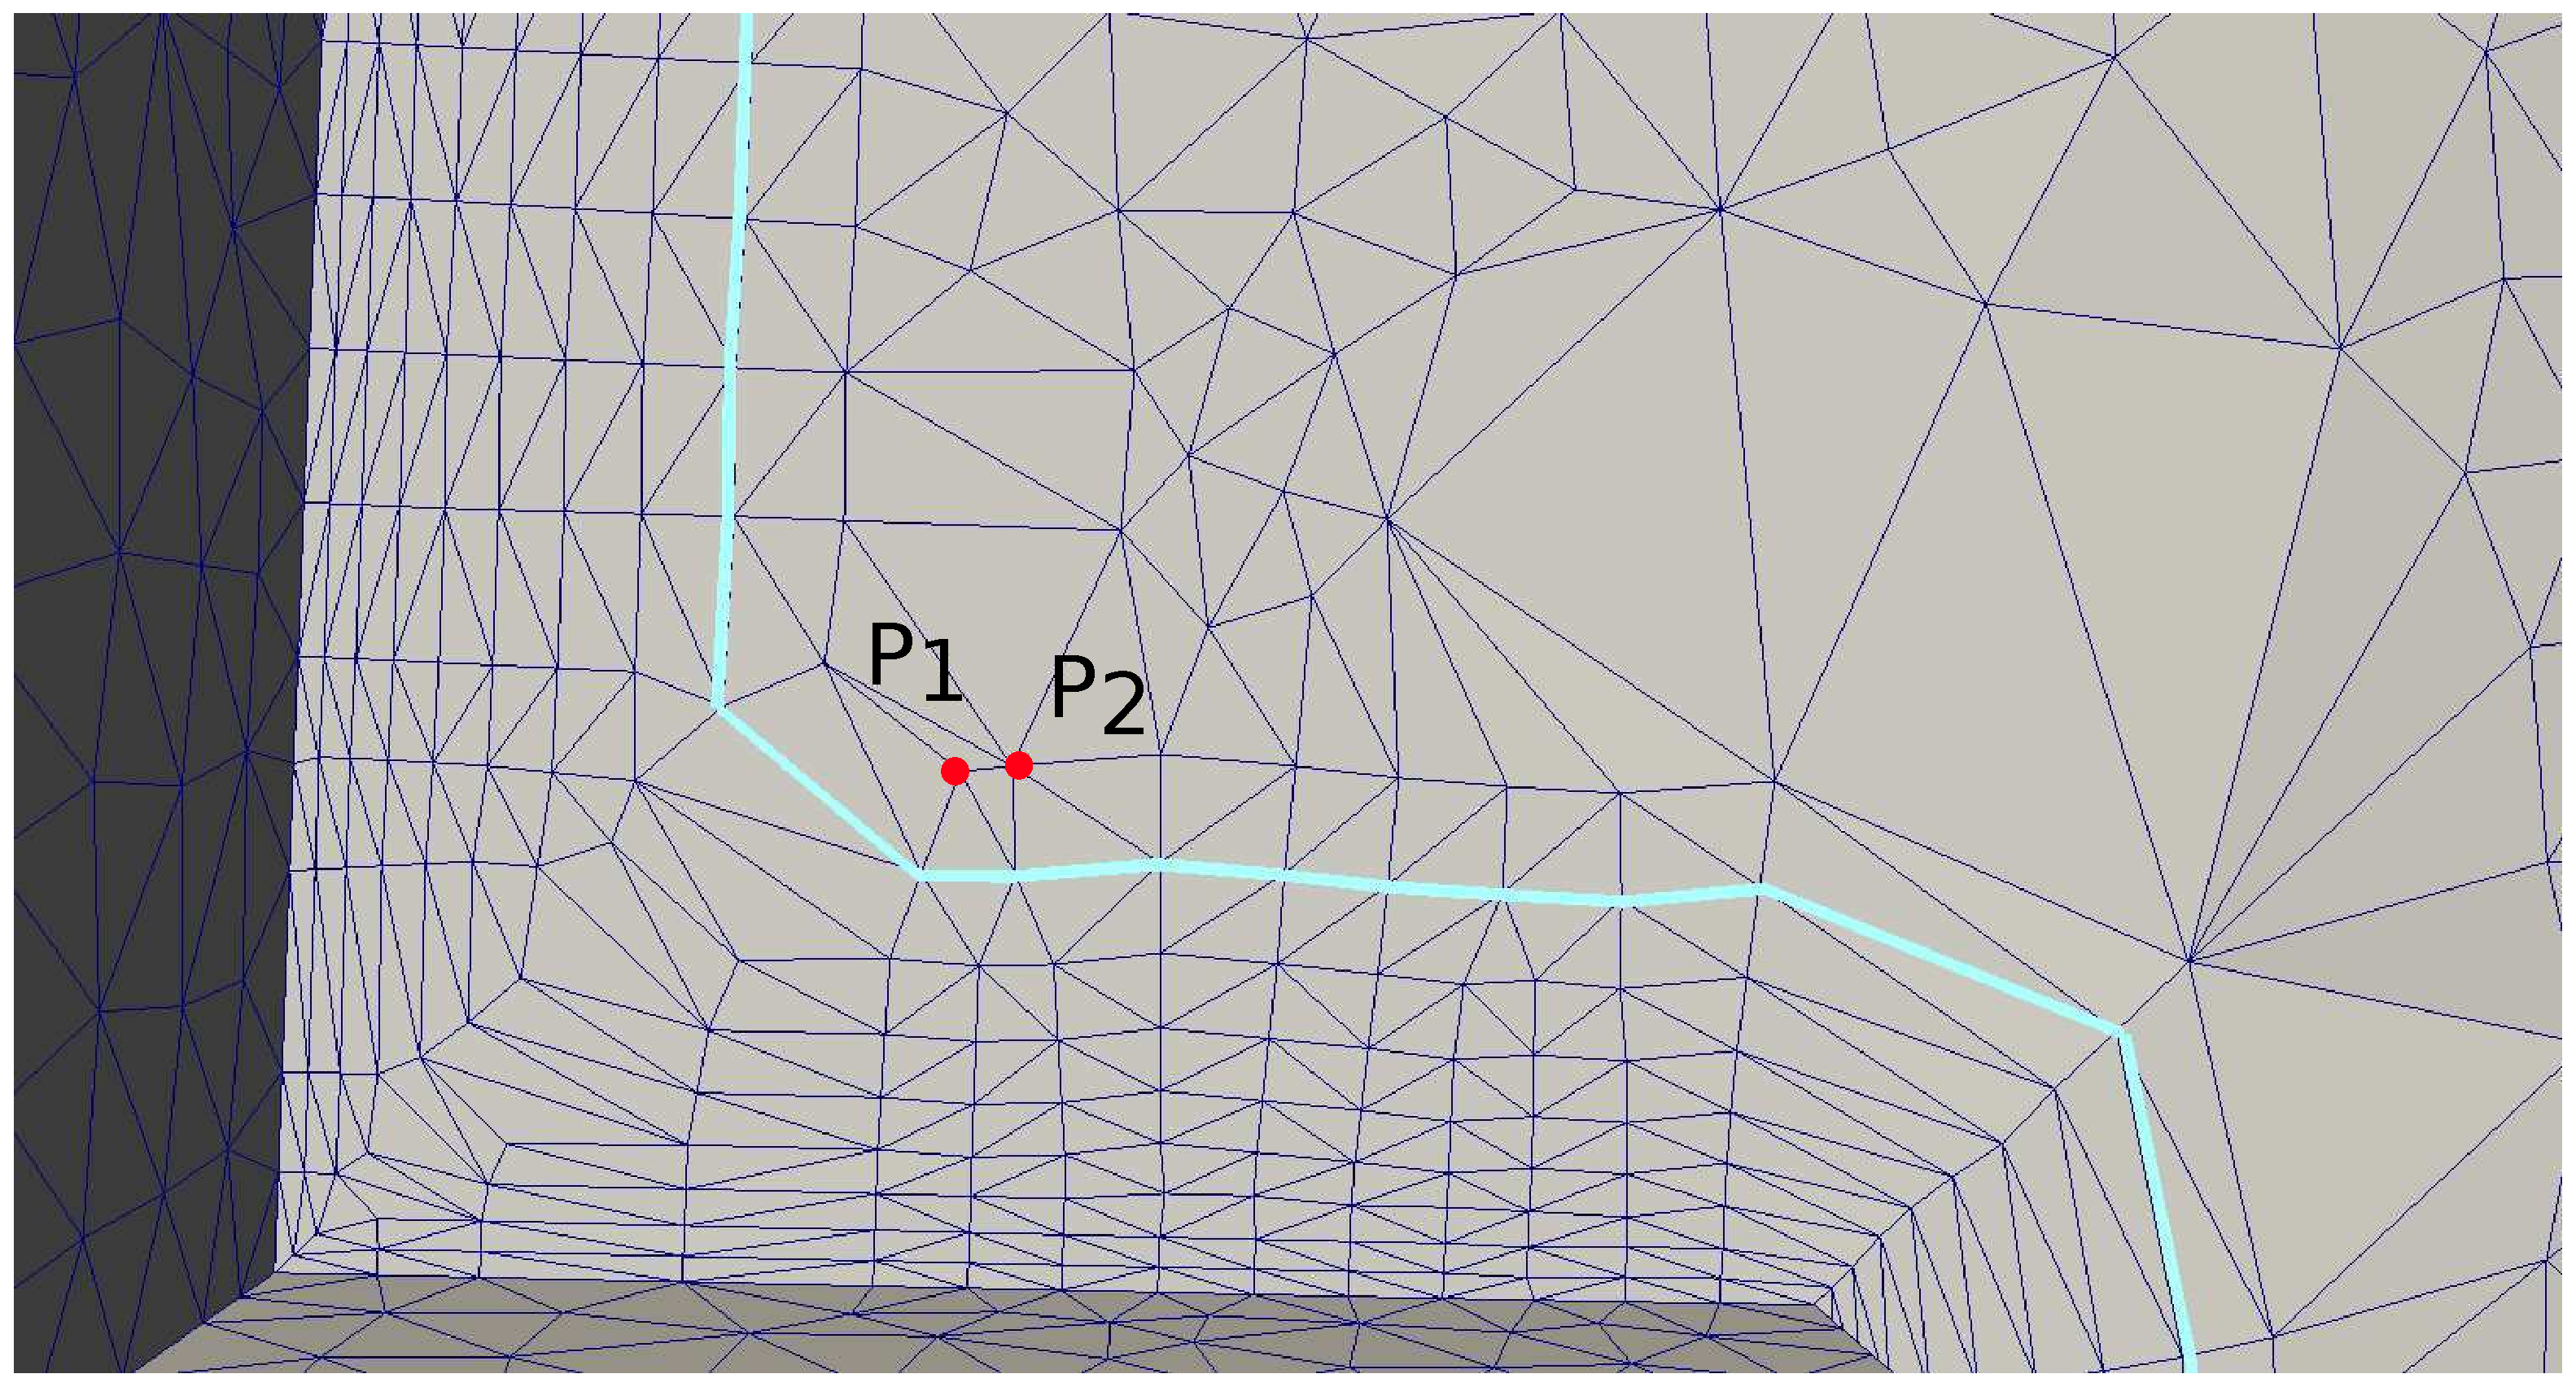
\includegraphics[width=.9\linewidth]{img/m2/edge-collapse/collapse1.eps}
  \caption{}
  \label{collapse1}
\end{subfigure}%
\begin{subfigure}{.5\textwidth}
  \centering
  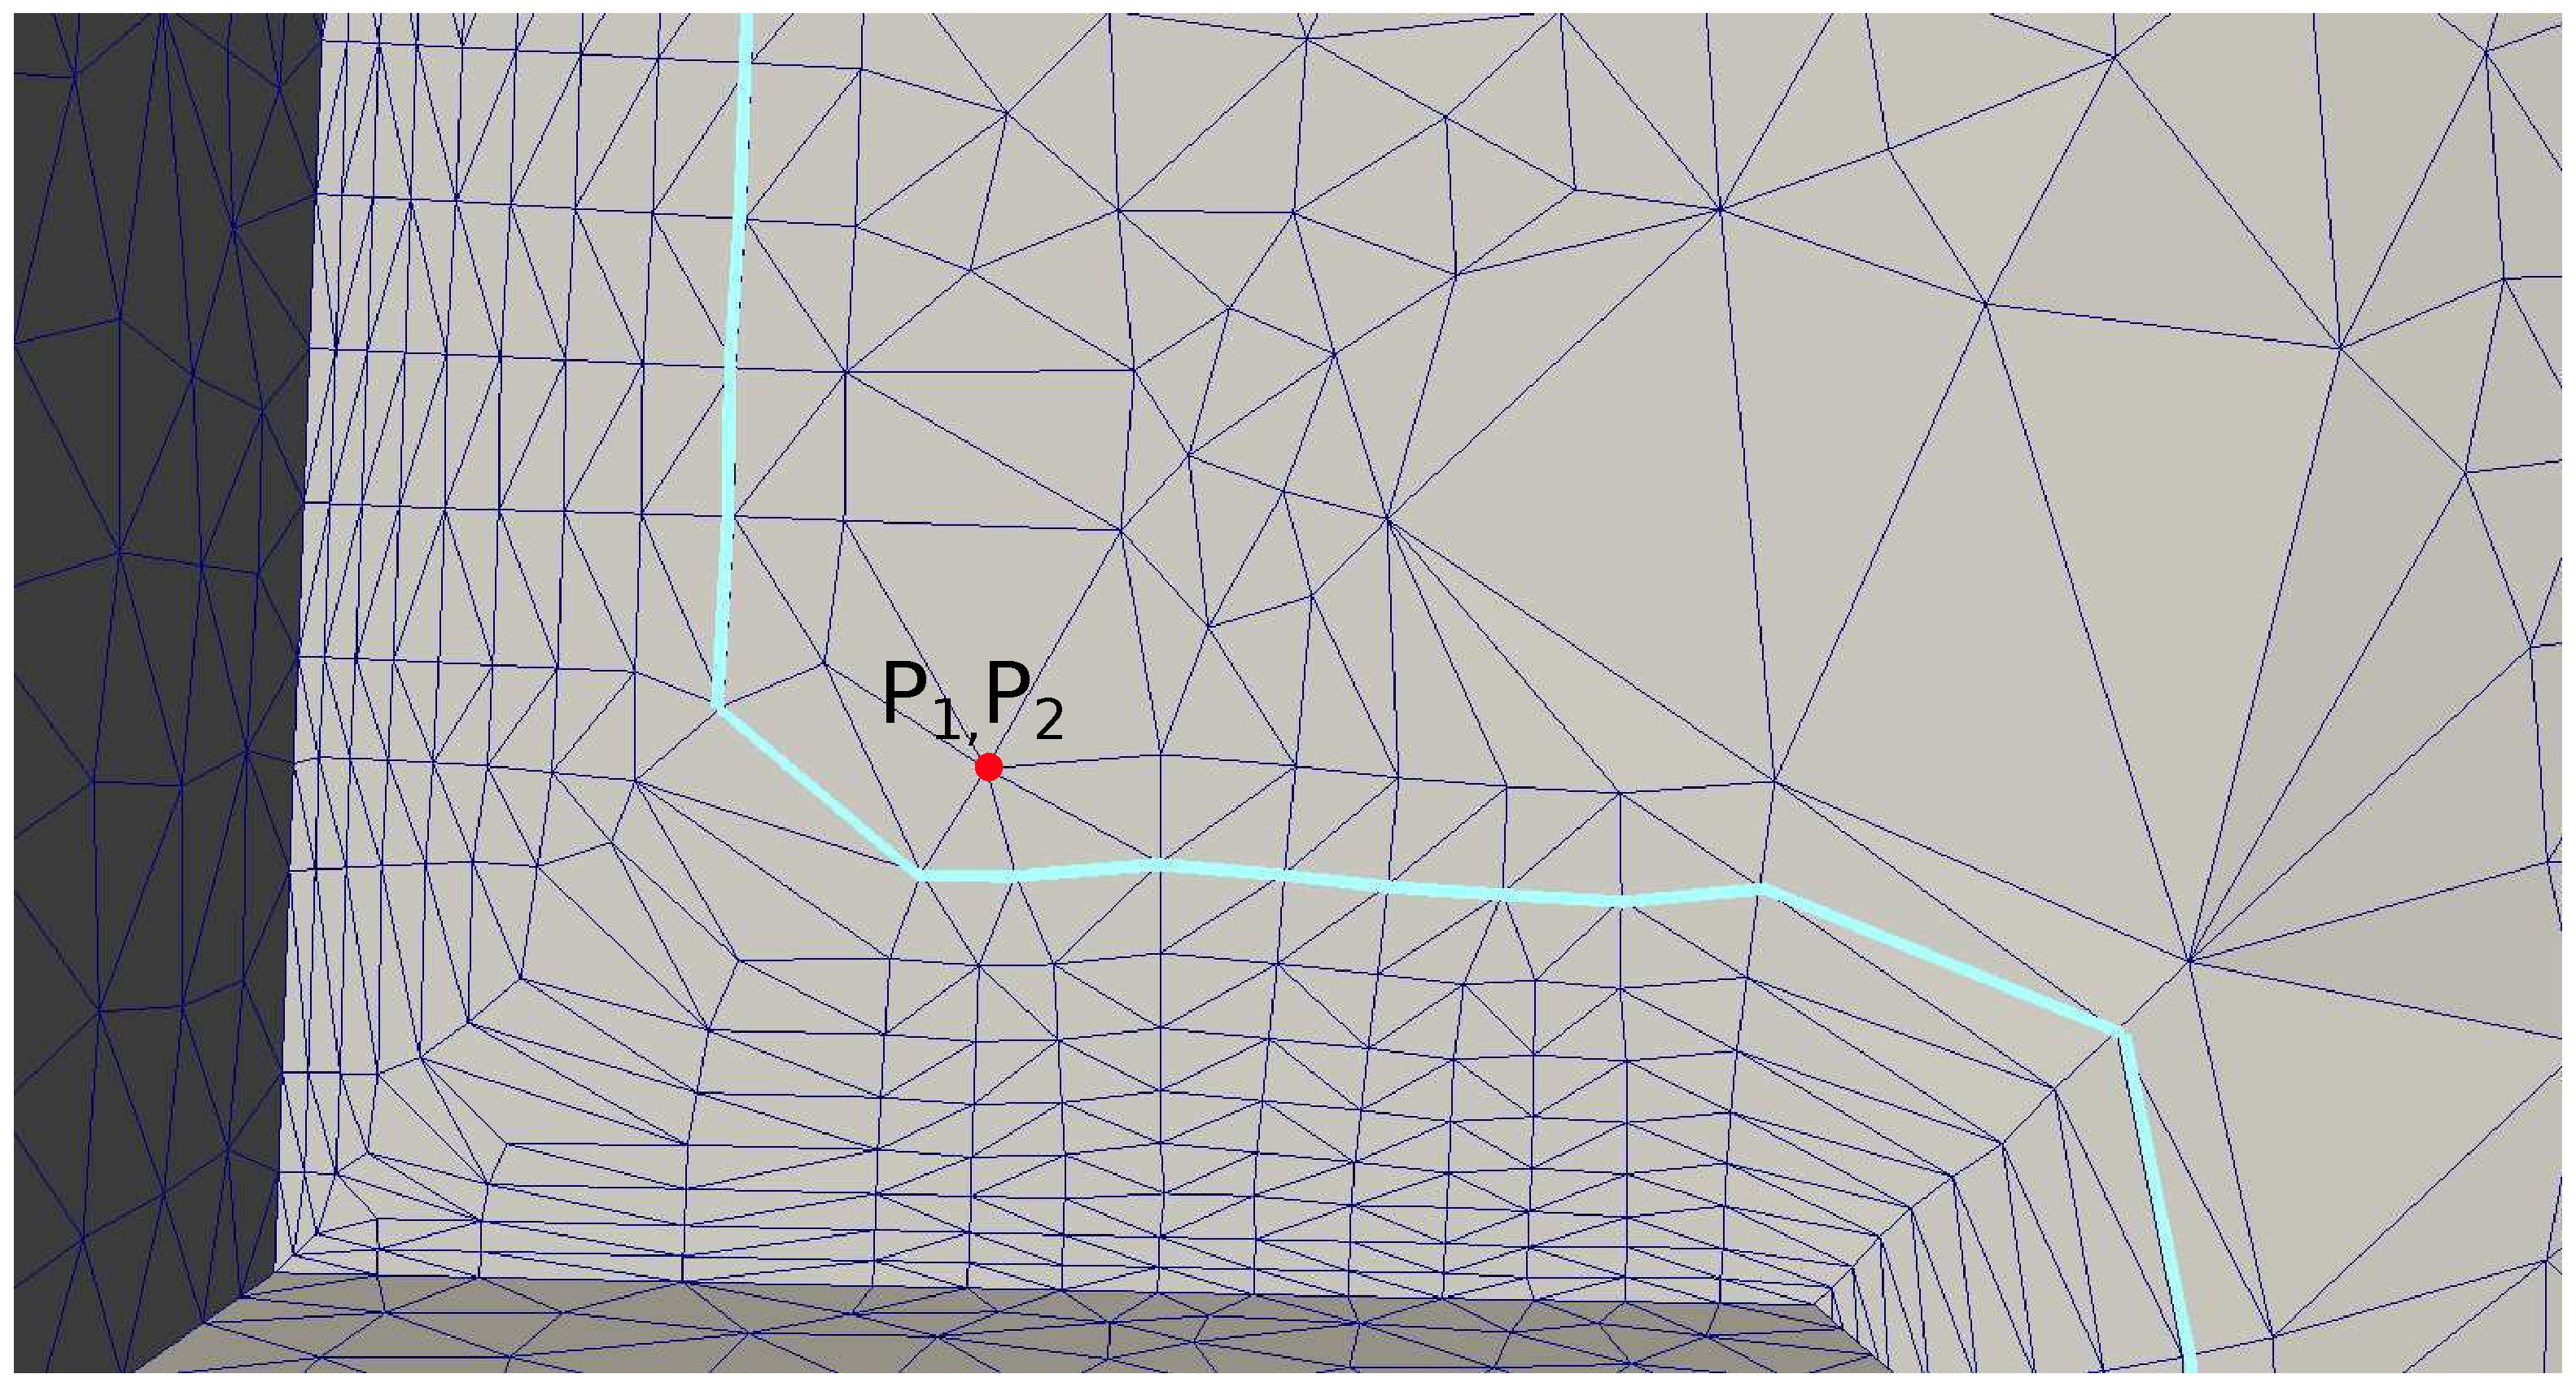
\includegraphics[width=.9\linewidth]{img/m2/edge-collapse/collapse2.eps}
  \caption{}
  \label{collapse2}
\end{subfigure}
\begin{subfigure}{.5\textwidth}
  \centering
  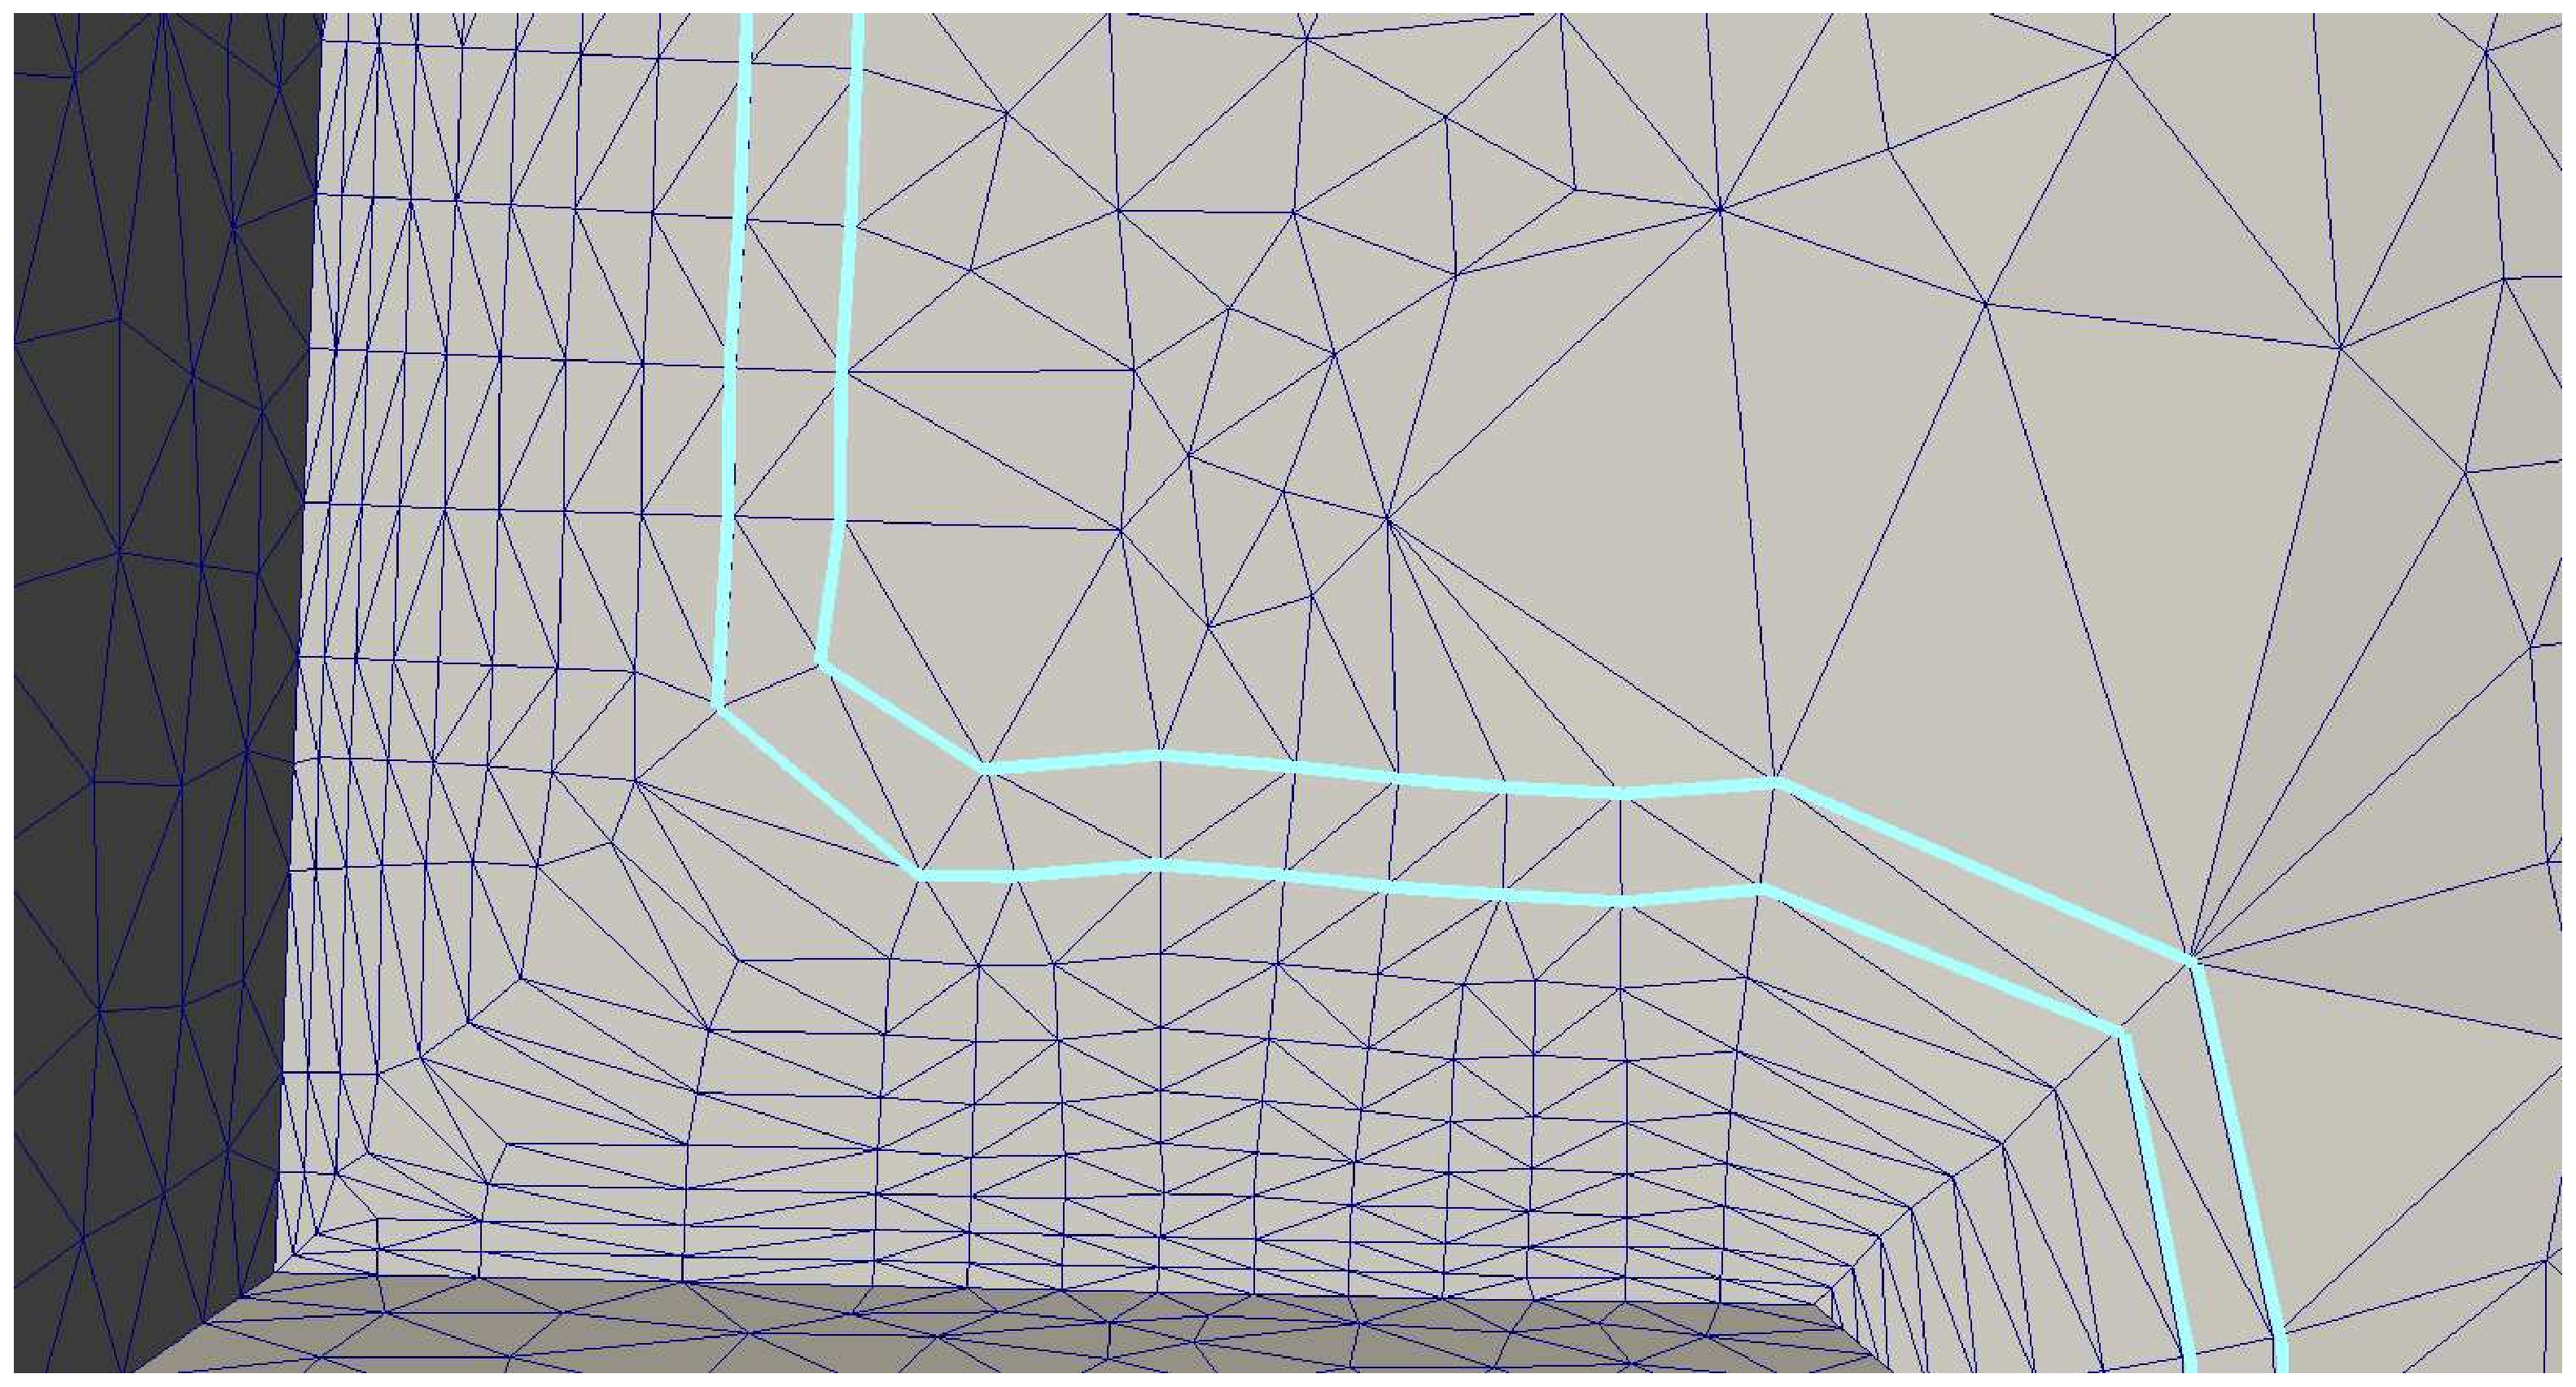
\includegraphics[width=.9\linewidth]{img/m2/edge-collapse/collapse3.eps}
  \caption{}
  \label{collapse3}
\end{subfigure}
\caption{Edge collapse on an advancing front to avoid encroachment of points. In (a), two points in the kid layer $P_1$ and $P_2$ are sufficiently close to each other. Their parent layer is highlighted. If both the points advance to the next layer, then the next front would fail to recover. Hence, the edge between them is chosen to collapse. (b) shows the result of the edge collapse. The new location of both the points is the average position of their initial location. (c) shows how the next front looks like.}
\label{edge-collapse}
\end{figure}

Once we have recovered the advancing front by iterative edge swaps to connect the kid points in the mesh, we check for vertices on the front that are too close to each other relative to the extrusion length. For instance, vertices which are near a concave corner could encroach each other if they are not decimated. Another example would be vertices on the advancing front which are far away from surface boundaries because the extrusion length has grown by this point. Decimating vertices from the front which are at a substantial distance from surface boundaries helps prevent the cell aspect ratio, ie front edge length over extrusion length, from dropping below one.

To check for vertices to decimate, we iterate through the vertices in the front and identify the ones which are too close to their neighbours. Vertex decimation is done through the edge-collapse routine as described in \cite{hoppe1994mesh}. The threshold edge length between two points on the front is set to be $2 \tan(\pi/8)$ times the average extrusion length at those points. This value is set so as to minimize the normalized maximum deviation of angle from $90^\circ$ for quad elements. Hence, the threshold ensures that the anisotropic properties are retained for several layers into the surface. All short edges on the front are collapsed using the edge-collapse algorithm. An example of an edge-collapse on the front is shown in Figure \ref{edge-collapse}. Here, two points $P_1$ and $P_2$ are collapsed into a single point which forms a part of the next front on the surface. Validation checks are made before collapsing an edge. The resultant triangles should not have a deviations of more than $50^{\circ}$ from the underlying surface.

As the advancing front marches into the surface, vertices in the interior of the surface immediately next to the front are decimated to make way for the advancing layers. Before extruding a point on the advancing front, we check if any point in the surface interior with which it shares an edge agrees with the following condition. If it does, we decimate the interior vertex.

\begin{equation}
    d < max \left(l_{1}/\sqrt{2}, \, l_{2}/\sqrt{2}, \, c\times \mathit{extrudeLength}\right)
    \label{collapse-eq}
\end{equation}

Here $d$ is the distance between the point on the advancing front and the interior point, $l_1$ and $l_2$ are the lengths of adjacent edges of the point on the front, c is a constant whose value is set as $2$ and $extrudeLength$ is the extrusion length at the vertex on the front. This condition ensures decimation of vertices in the surface interior which are close to the advancing front and avoids any encroachment of surface interior vertices on the advancing layers. Topological and geometrical checks are done before an edge can be collapsed. These include a threshold for the ratio of area of generated triangles and a limit on the dihedral angle between the adjacent triangles created by the collapse. The area threshold is set to be $10^8$. Also, edge-collapse is successful only if the triangles resulting from it are be within a limit of $\theta < 30^{\circ}$ from the surface(see Figure \ref{deviation-surface}). The threshold for the maximum dihedral angle between any two adjacent triangles that result from the edge-collapse is set to $40^{\circ}$. The quality criterion used for edge collapse is again maximization of the minimum angle in the triangles thus produced. The best edge for collapse is chosen when decimating the interior vertices using this quality criterion. This is in contrast to the vertex decimation on the advancing front where the candidate edge for collapse is already identified. An illustrative example for surface interior vertex decimation can be seen in Figure \ref{interior-vert-collapse}.

After we have a recovered the front and decimated encroaching vertices in the surface interior as well as on the advancing front through edge collapse, we queue up the immediate interior edges of the surface and swap them for maximizing mesh quality. This step is included so that we have a good interior triangulation at each step of the advancing layer routine. This step ensures that we do not have bad triangles causing problems as we continue to march.

\begin{figure}[hbt!]
\centering
\begin{subfigure}{.5\textwidth}
  \centering
  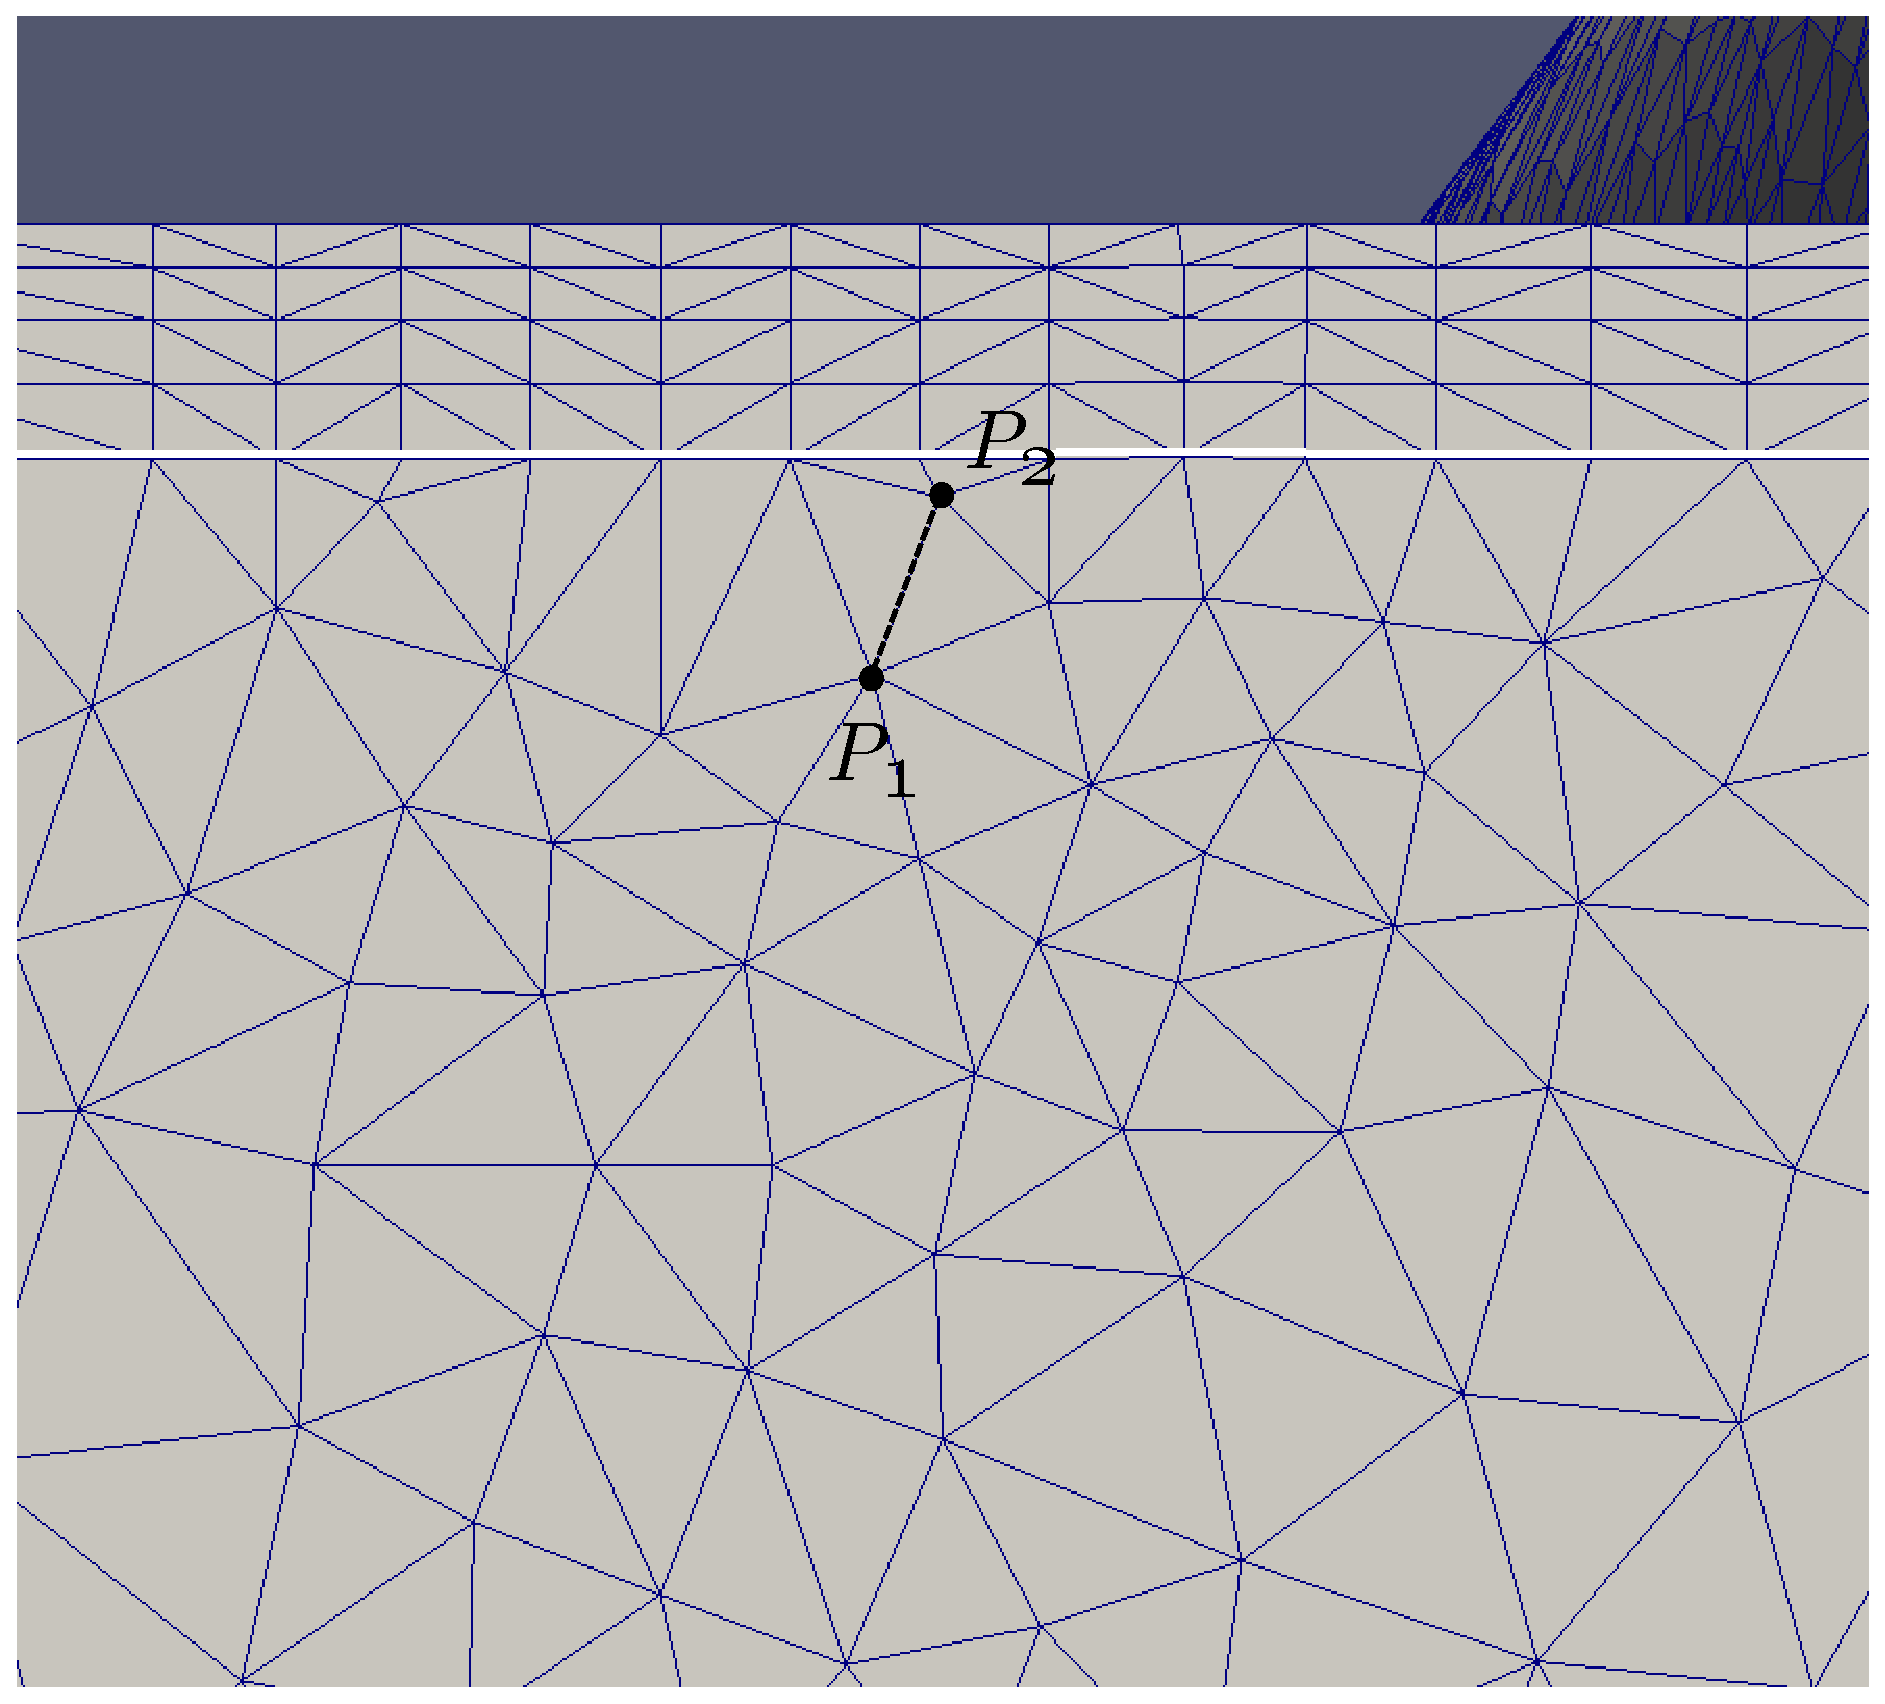
\includegraphics[width=.9\linewidth, trim={0 5cm 0  0}, clip]{img/m2/interior-vert-collapse/cc1.eps}
  \caption{}
  \label{cc1}
\end{subfigure}%
\begin{subfigure}{.5\textwidth}
  \centering
  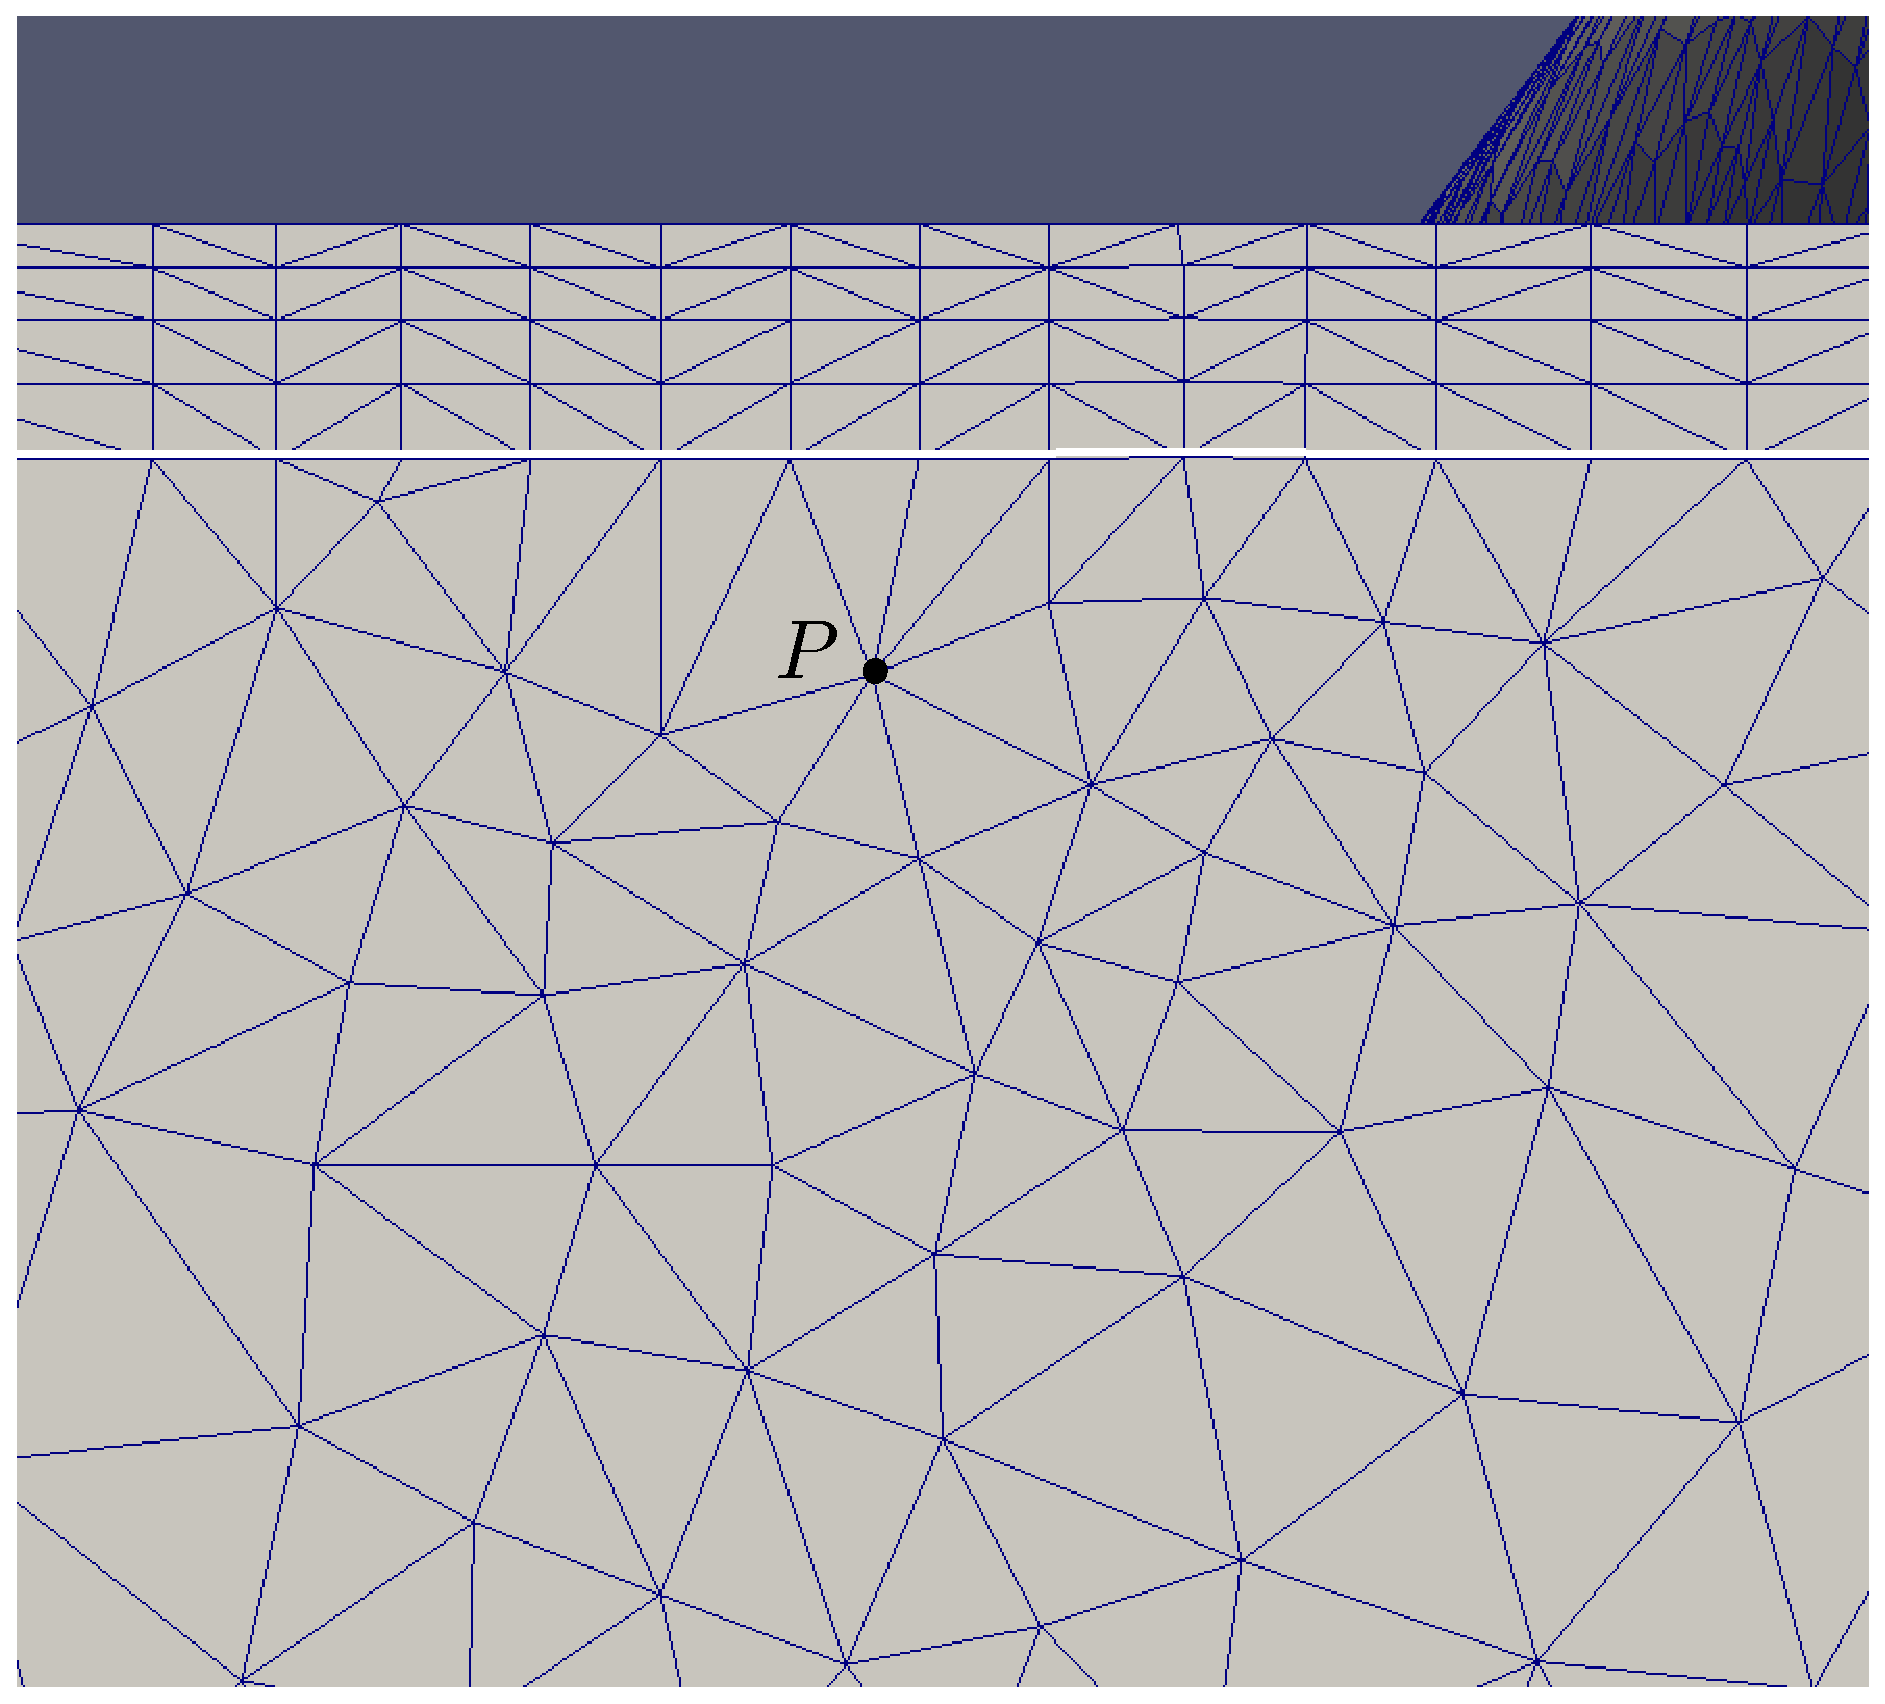
\includegraphics[width=.9\linewidth, trim={0 5cm 0  0}, clip]{img/m2/interior-vert-collapse/cc2.eps}
  \caption{}
  \label{cc2}
\end{subfigure}
\begin{subfigure}{.5\textwidth}
  \centering
  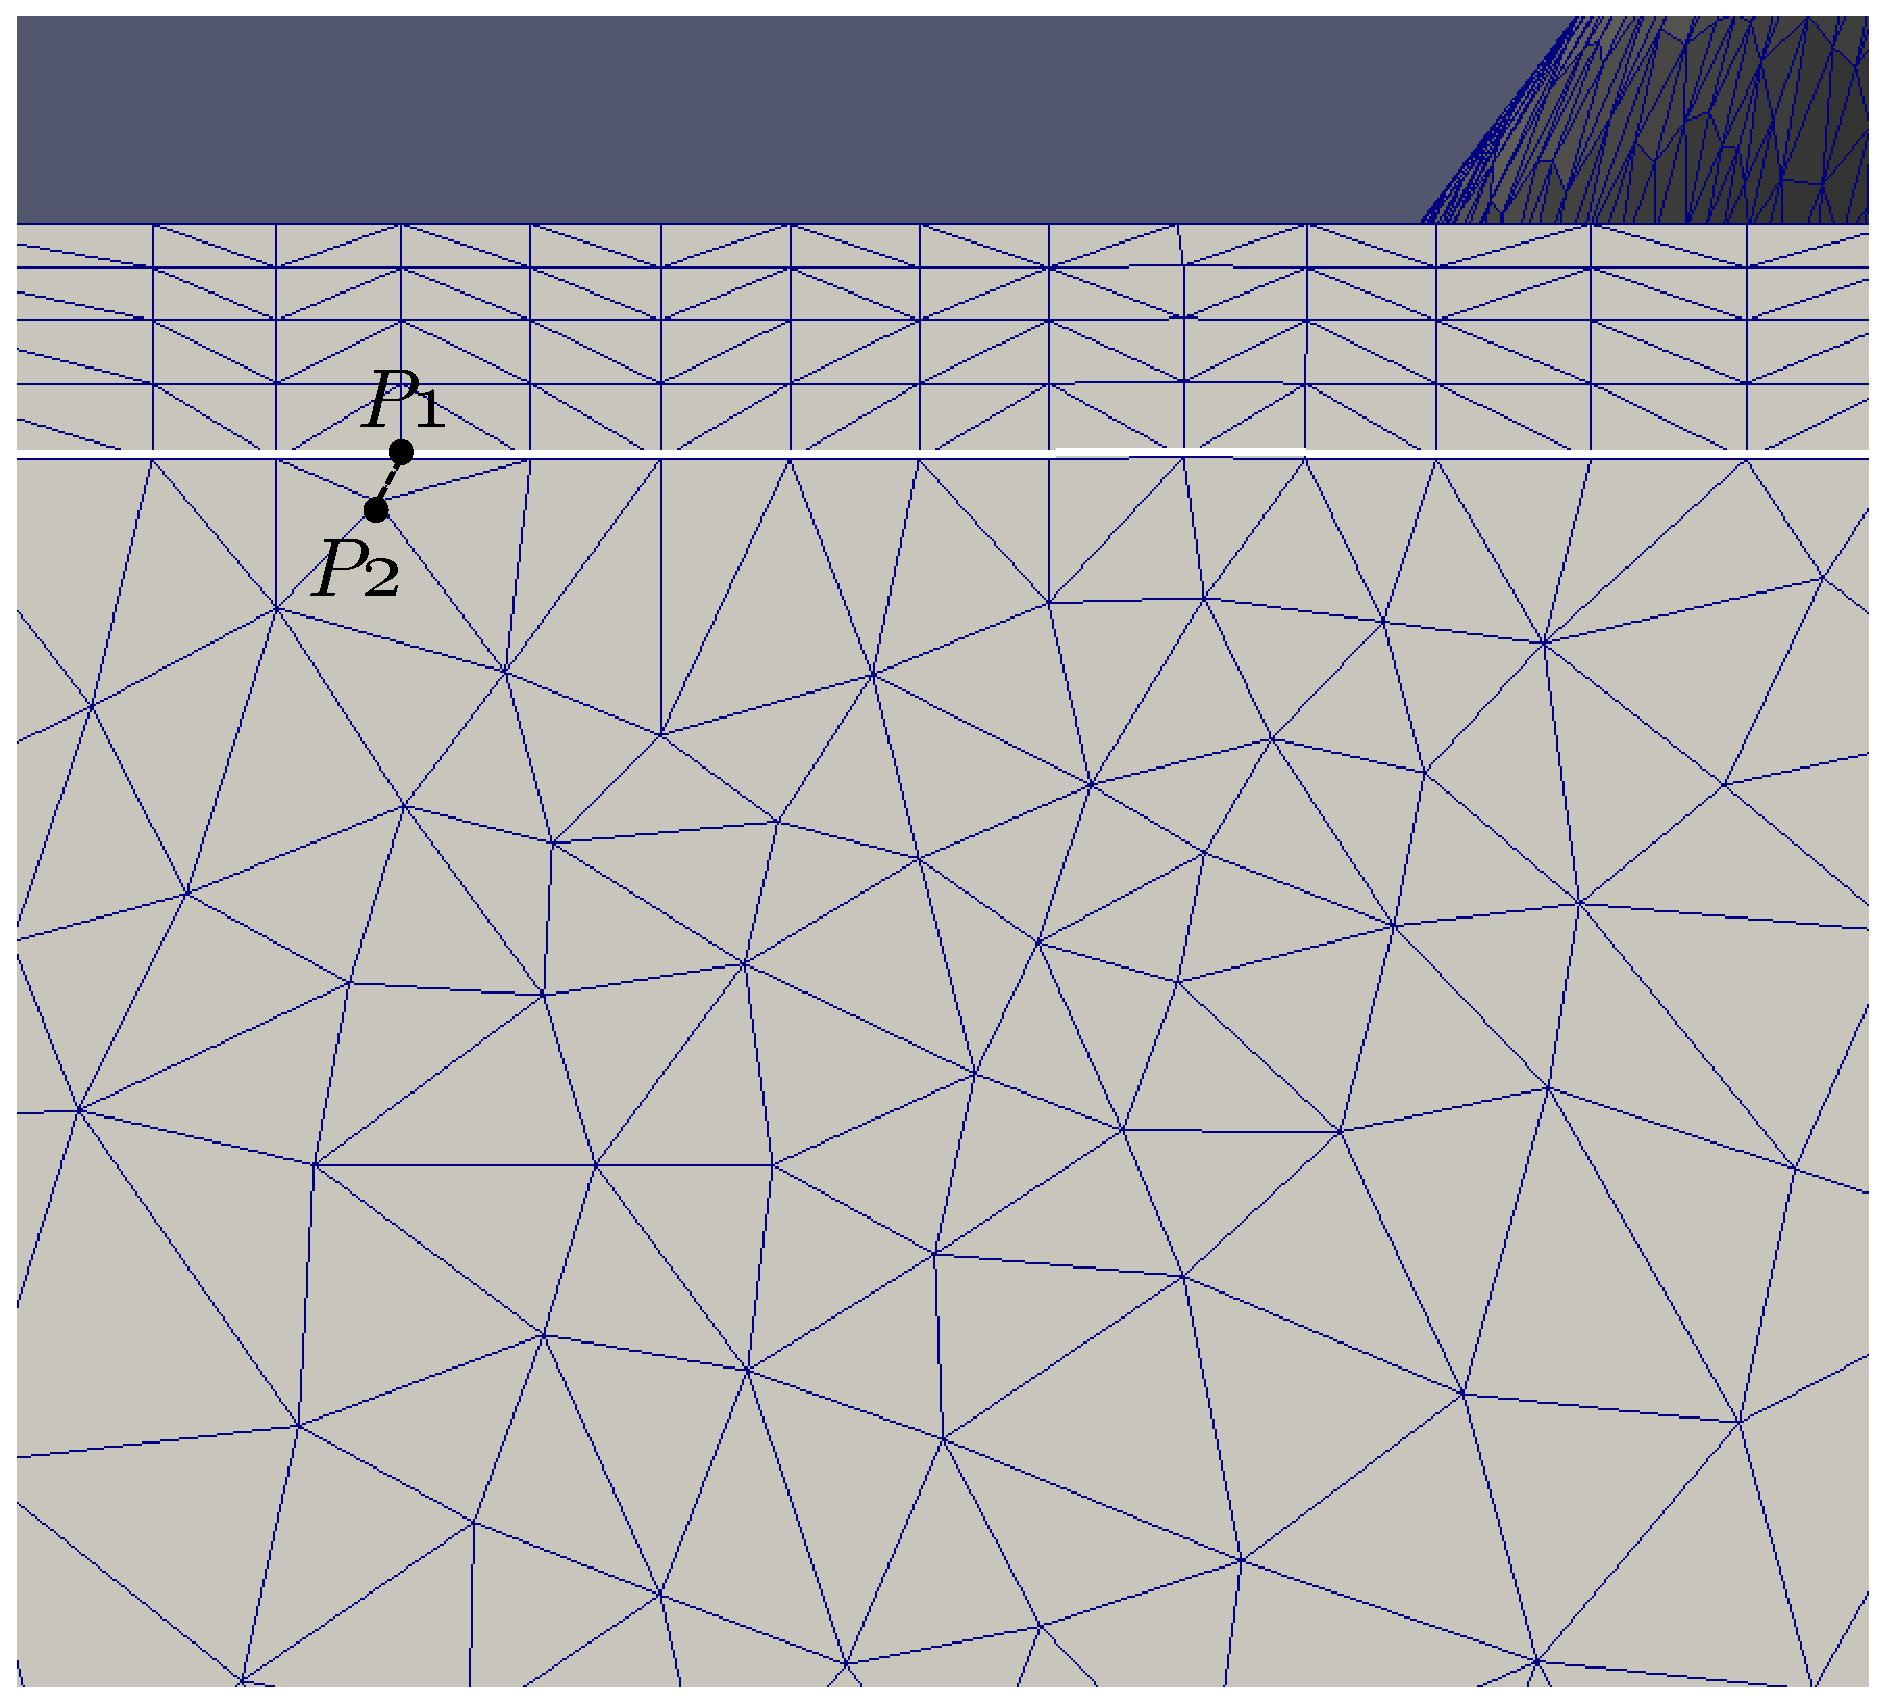
\includegraphics[width=.9\linewidth, trim={0 5cm 0  0}, clip]{img/m2/interior-vert-collapse/cc3.eps}
  \caption{}
  \label{cc3}
\end{subfigure}%
\begin{subfigure}{.5\textwidth}
  \centering
  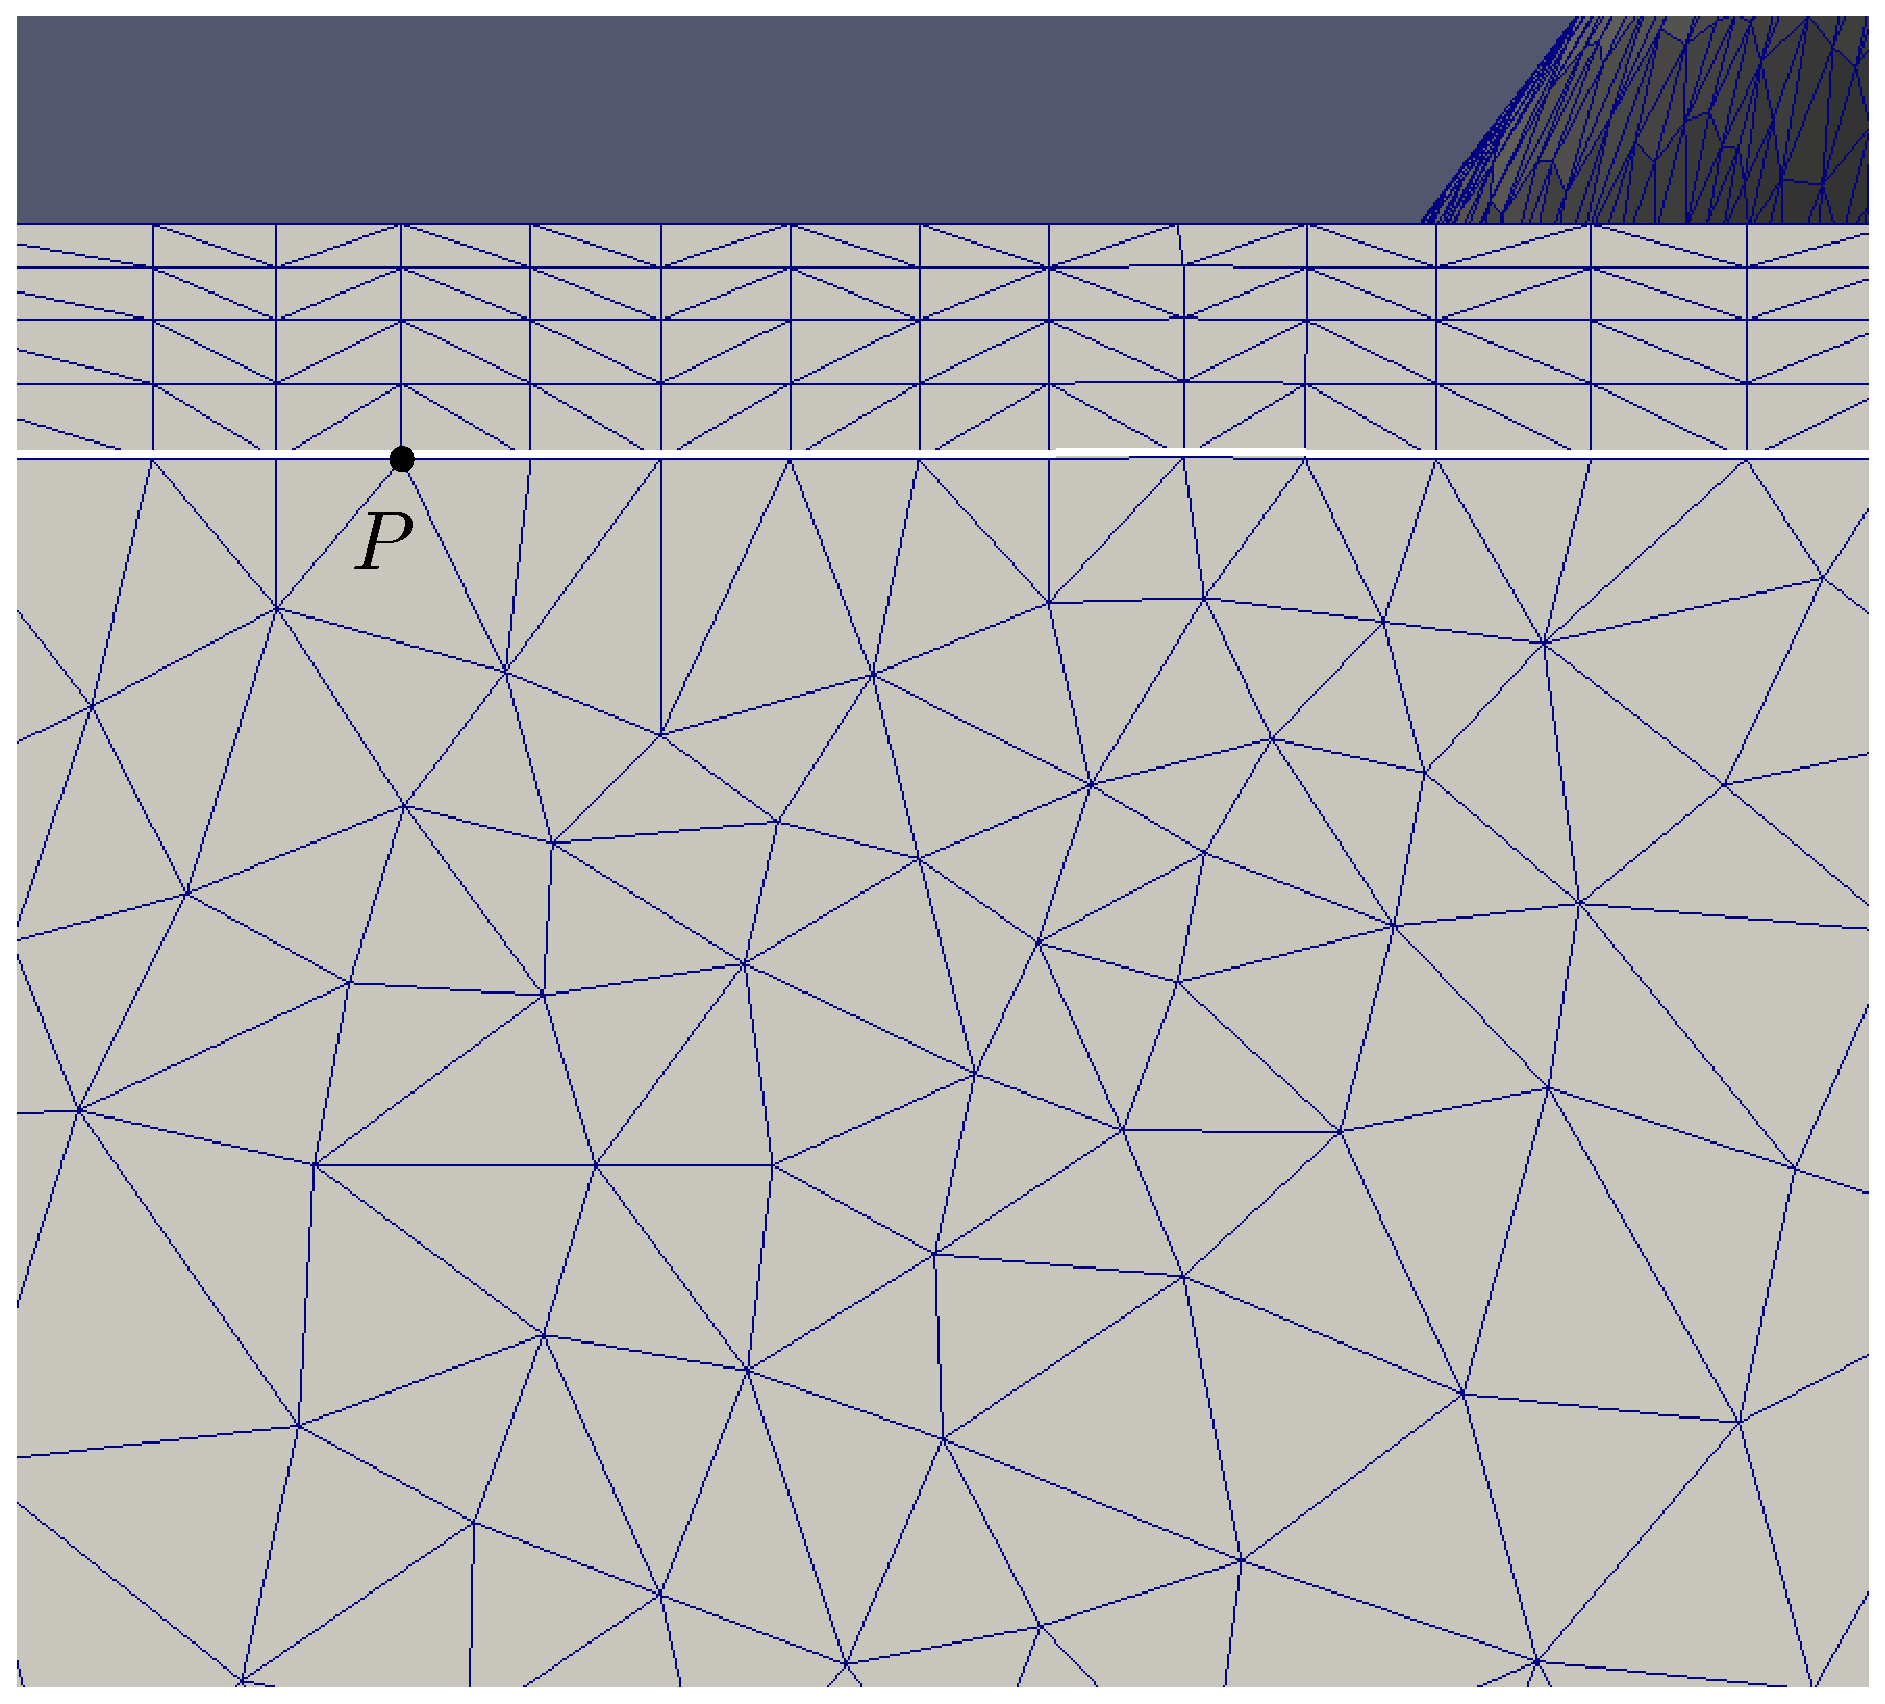
\includegraphics[width=.9\linewidth, trim={0 5cm 0  0}, clip]{img/m2/interior-vert-collapse/cc4.eps}
  \caption{}
  \label{cc4}
\end{subfigure}
\caption{Interior vertex decimation through edge collapse. The highlighted line shows the advancing front. In (a), vertex $P_2$ is about to encroach the front. Hence, the best vertex for collapse is chosen among its neighbours. The best vertex for edge collapse here is $P_1$. Hence, $P_2$ is collapsed on to $P_1$. The connectivity after the edge collapse is shown in (b) where vertex $P$ represents the collapsed vertex. Similarly, in (c), vertex $P_2$ is about to encroach the advancing front and is collapsed onto vertex $P_1$ which is on the advancing front itself. The new connectivity is shown in (d) where all the possibly encroaching vertices for the advancing layer are decimated.}
\label{interior-vert-collapse}
\end{figure}
